\documentclass[11pt]{article}

\usepackage[margin=1in]{geometry}
\usepackage{amsmath, amssymb}
\usepackage{graphicx}
\usepackage{booktabs}
\usepackage{hyperref}
\usepackage{caption}
\usepackage{subcaption}

\title{Model Comparison on the Cylinder Graph HMM}
\author{Claude \& C. L.}
\date{\today}

\begin{document}
\maketitle

%----------------------------------------------------------------------
\section{Problem Setup}
%----------------------------------------------------------------------

We consider a Hidden Markov Model (HMM) whose hidden-state graph has the
topology of a discrete cylinder.  The cylinder has \emph{width}
$n = 6$ (nodes per level) and \emph{depth} $D = 3$ (number of levels),
giving $n \times D = 18$ hidden states in total.

\paragraph{Transition structure.}
From a node $(l, j)$ at depth $l$ and angular position $j$ the chain can
jump to three neighbours:
\begin{itemize}
  \item \textbf{Nearest neighbour (NN):} $(l,\, j{+}1 \bmod n)$ with
        weight $w \sim \mathrm{Uniform}(0, 1-p)$;
  \item \textbf{Next-nearest neighbour (NNN):} $(l,\, j{+}2 \bmod n)$
        with weight $1 - p - w$;
  \item \textbf{Next layer:} $((l{+}1) \bmod D,\, j)$ with fixed
        probability $p = 0.1$.
\end{itemize}
The intra-layer weights are drawn once at initialisation (seed 42) and
held fixed thereafter; the inter-layer probability $p$ controls how
often the chain cycles through the depth levels.

\paragraph{Emission structure.}
The vocabulary has $|V| = D \times K = 3 \times 16 = 48$ tokens,
partitioned into three clusters of 16 tokens each (one cluster per depth
level).  Each hidden state at depth $l$ emits tokens only from cluster
$l$, with emission probabilities drawn from a symmetric Dirichlet
distribution with concentration parameter $\alpha = 0.3$.  The small
$\alpha$ makes the per-state distributions sparse, so different states
at the same depth emit noticeably different token profiles.

\paragraph{Entropy rate.}
The theoretical (Shannon) entropy rate of the process, estimated via a
long Monte-Carlo trajectory, is
\begin{equation}
  h \;\approx\; 2.4396 \;\text{nats/token}.
\end{equation}
This serves as the information-theoretic lower bound on the
cross-entropy loss achievable by any predictor.

%----------------------------------------------------------------------
\section{Transformer Architectures}
%----------------------------------------------------------------------

We train causal transformer language models (implemented via
TransformerLens \texttt{HookedTransformer}) to predict the next token in
sequences of length $T = 16$ generated by the cylinder HMM.

The hyperparameter sweep covers:
\begin{center}
\begin{tabular}{ll}
  \toprule
  Hyperparameter & Values \\
  \midrule
  Number of layers $L$        & 2, 4 \\
  Embedding dimension $d$     & 4, 8, 16, 32, 48, 64 \\
  Number of heads $H$         & 1, 2, 4 \\
  Architecture                & attention-only, full (attention + MLP) \\
  Normalisation               & none, LayerNorm \\
  \bottomrule
\end{tabular}
\end{center}
All models use ReLU activations, tied input/output embeddings, and
$d_{\mathrm{mlp}} = 4d$ for full architectures.  Training uses AdamW
($\beta_1 = 0.9$, $\beta_2 = 0.999$, weight decay $0.01$, learning rate
$10^{-3}$) with batch size 128 for 10 epochs.  A total of 135 models
were trained on a dataset of ${\sim}\,618\text{k}$ sequences
($10^7$ tokens).

%----------------------------------------------------------------------
\section{Results: Model Size vs.\ Validation Loss}
%----------------------------------------------------------------------

Figure~\ref{fig:model-comparison} plots the best validation loss
achieved by each model against its parameter count.

\begin{figure}[htbp]
  \centering
  \begin{subfigure}[t]{0.48\textwidth}
    \centering
    
\includegraphics[width=\textwidth]{model_comparison.png}
    \caption{Validation loss vs.\ parameter count.  Circles: attention-only;
             squares: full (attention + MLP).  Blue: LayerNorm; red: no
             normalisation.  Dashed lines mark the theoretical entropy rate
             $h \approx 2.44$\,nats/token and the Bayes-optimal loss
             $L^{*}(k{=}16)$.}
    \label{fig:model-comparison-abs}
  \end{subfigure}
  \hfill
  \begin{subfigure}[t]{0.48\textwidth}
    \centering
    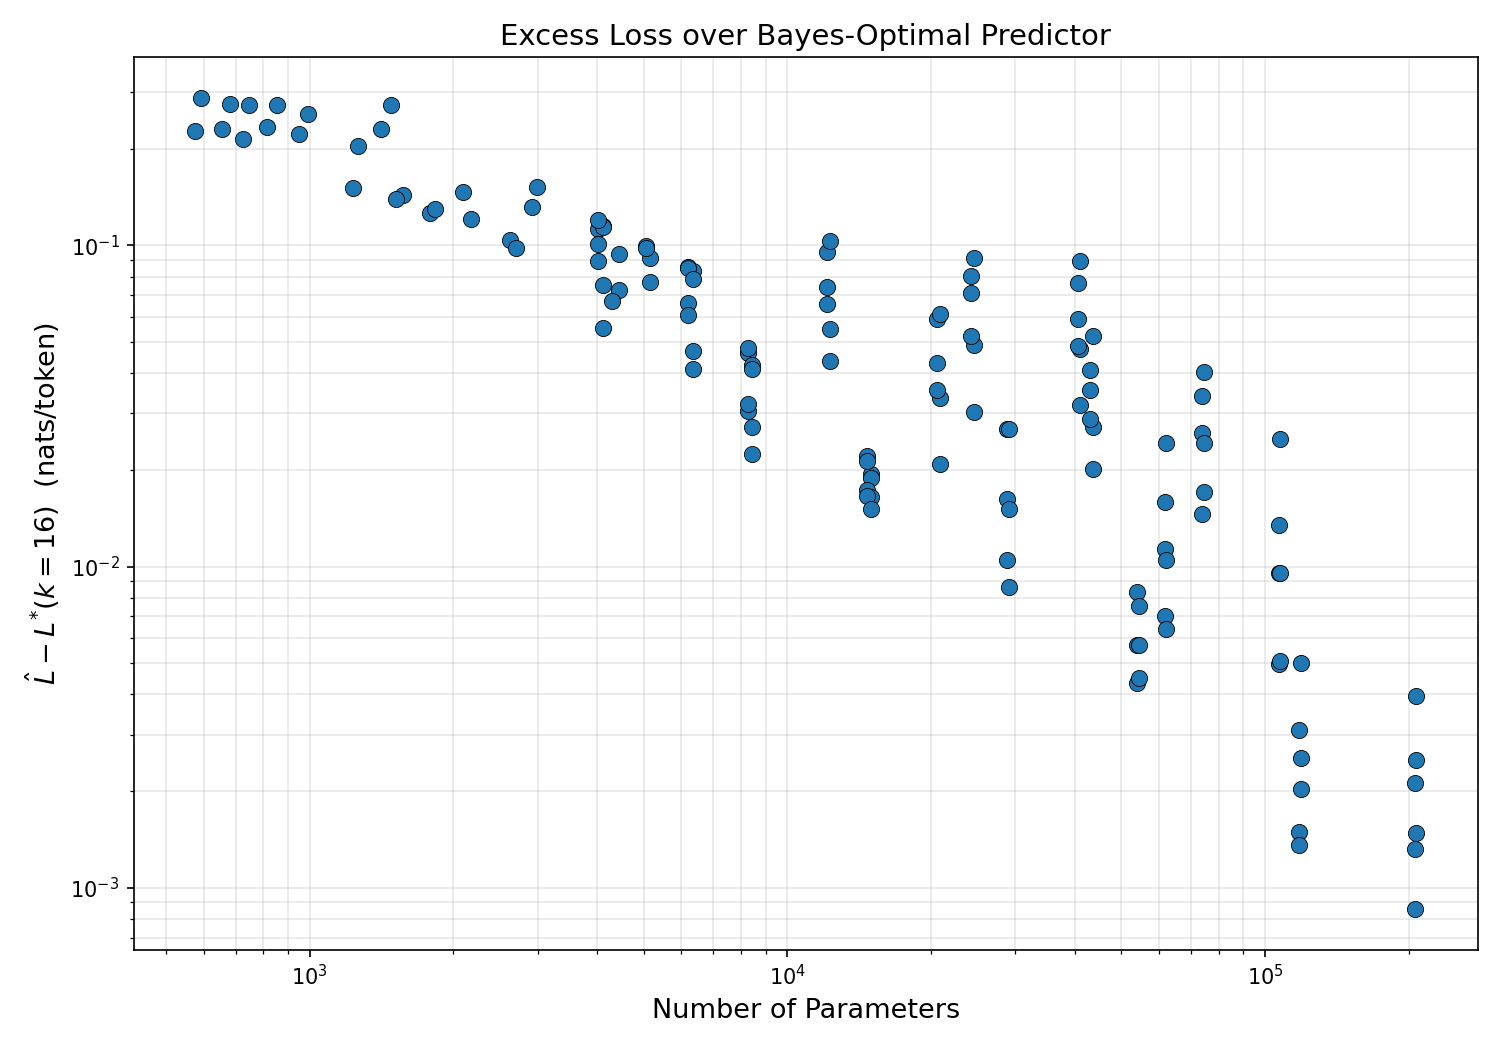
\includegraphics[width=\textwidth]{excess_loss_loglog.png}
    \caption{Excess loss $\hat{L} - L^{*}(k{=}16)$ on a log--log scale.
             All architectural distinctions are suppressed to highlight
             the overall scaling trend with model size.}
    \label{fig:model-comparison-excess}
  \end{subfigure}
  \caption{Model size versus validation loss for 135 transformer
           configurations on the Cylinder Graph HMM\@.
           (a)~Absolute validation loss.
           (b)~Excess loss over the Bayes-optimal predictor at context
           length~$k = 16$.}
  \label{fig:model-comparison}
\end{figure}

Key observations:
\begin{enumerate}
  \item \textbf{Scaling with model size.}  Validation loss decreases
        roughly log-linearly with parameter count up to
        ${\sim}10^5$ parameters, after which gains diminish.
  \item \textbf{Full $>$ attention-only.}  At every scale the full
        transformer (with MLP layers) outperforms its attention-only
        counterpart, consistent with the MLP layers' role in
        implementing nonlinear token-mixing needed to approximate
        posterior belief updates.
  \item \textbf{Layer norm is approximately neutral.}  LayerNorm and
        no-LayerNorm models achieve similar best losses; the effect is
        secondary to architecture and scale.
  \item \textbf{Gap to entropy rate.}  The best model
        (L4, $d{=}64$, $H{=}4$, full, no-LN; ${\sim}206$k parameters)
        reaches a validation loss of ${\approx}\,2.473$\,nats/token,
        roughly $0.034$\,nats above the theoretical entropy rate.  This
        residual gap likely reflects the finite context window ($T = 16$)
        and architectural limitations in representing exact belief-state
        inference.
  \item \textbf{Depth helps.}  All top-10 models use $L = 4$ layers,
        suggesting that additional depth is beneficial for tracking the
        hidden-state posterior across multiple emission steps.
\end{enumerate}

\paragraph{Log likelihood ratio tests.}
To evaluate the ability of the model in predicting the next token, we
compare between:
\begin{enumerate}
  \item The true next-token prediction, computing the exact belief state
        at each step assuming a prior of the stationary distribution.
        Note that in this case we know the parameters of the HMM\@.
  \item The transformer model's prediction, where the log likelihood of
        the next token is extracted from the model's logits.
\end{enumerate}

%----------------------------------------------------------------------
\section{Embedding Structure}
%----------------------------------------------------------------------

Figure~\ref{fig:embedding} shows the cosine-similarity matrix and
$\ell_2$ norms of the learned token-embedding vectors from a
representative model.  The $3 \times 3$ block structure in the
similarity matrix directly mirrors the depth-level clustering of the
vocabulary: tokens within the same depth cluster are mapped to similar
embedding directions, while cross-cluster pairs are near-orthogonal or
anti-correlated.  This confirms that the model discovers the latent
depth structure without supervision.

\begin{figure}[htbp]
  \centering
  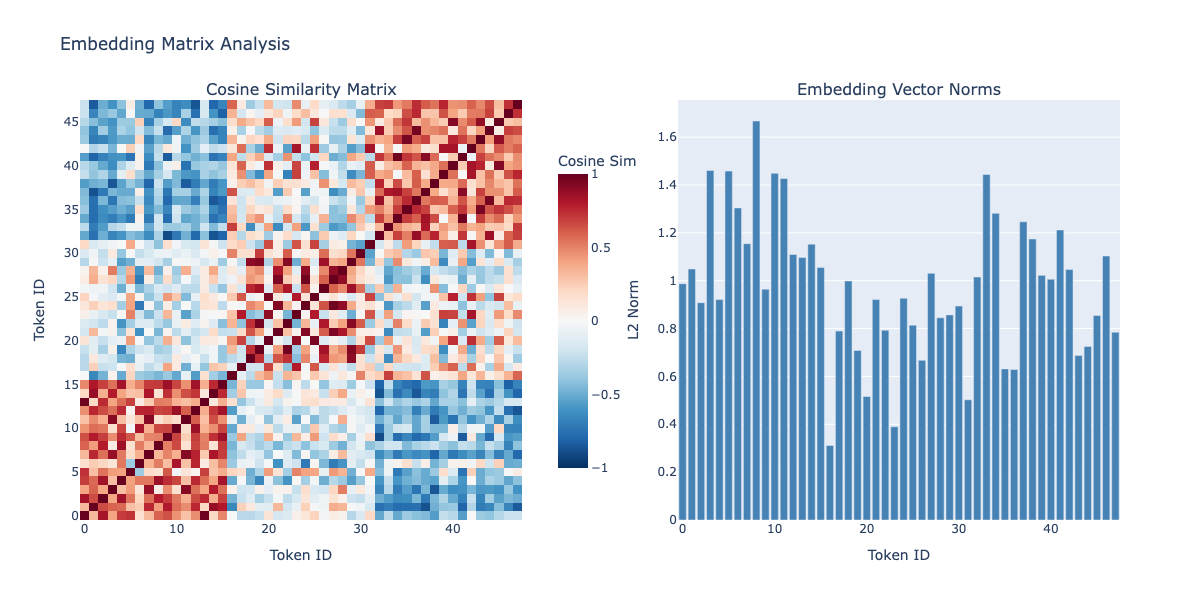
\includegraphics[width=0.85\textwidth]{newplot.png}
  \caption{Left: cosine similarity matrix of the $48 \times d$ embedding
           matrix.  The visible $3 \times 3$ block structure corresponds
           to the three depth levels.  Right: $\ell_2$ norm of each
           token's embedding vector.}
  \label{fig:embedding}
\end{figure}

\paragraph{Cluster similarity across architectures.}
To quantify how consistently the embedding geometry reflects the
depth-level structure, we compute the cosine similarity between cluster
centroids across all 135 trained models.  For each model we extract the
embedding matrix $W_E \in \mathbb{R}^{48 \times d}$ and compute three
centroids
\begin{equation}
  \mathbf{c}_l = \frac{1}{16}\sum_{v=16l}^{16l+15} W_E[v,:],
  \qquad l \in \{0,1,2\},
\end{equation}
followed by the three pairwise cosine similarities
$\mathrm{sim}(\mathbf{c}_0, \mathbf{c}_1)$,
$\mathrm{sim}(\mathbf{c}_0, \mathbf{c}_2)$, and
$\mathrm{sim}(\mathbf{c}_1, \mathbf{c}_2)$.

Figure~\ref{fig:cluster-sim} shows these similarities as a function of
validation loss.  All three pairs are predominantly negative
(mean $\approx -0.4$), confirming that the learned embeddings separate
the three depth clusters into roughly opposing directions in embedding
space.  Models that achieve low validation loss (left side of the plot)
cluster tightly in the range $-0.35$ to $-0.50$, while poorly
performing models exhibit much higher variance---some cluster pairs even
become positively correlated.  This suggests that learning to separate
the depth clusters in embedding space is necessary for good predictive
performance, but the degree of separation saturates once the model is
sufficiently expressive.

\begin{figure}[htbp]
  \centering
  \begin{subfigure}[t]{0.48\textwidth}
    \centering
    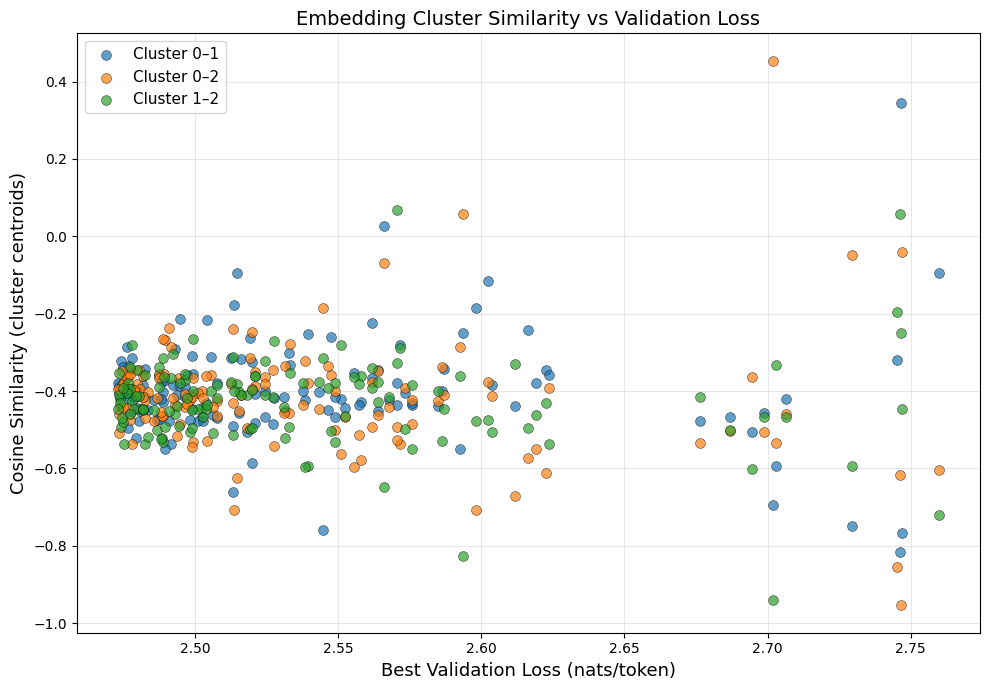
\includegraphics[width=\textwidth]{figures/embedding_cluster_similarity_raw.png}
    \caption{All three pairwise cosine similarities between cluster
             centroids, plotted for each of the 135 trained models.
             Poorly performing models show high variance, with some
             cluster pairs becoming positively correlated.}
    \label{fig:cluster-sim-raw}
  \end{subfigure}
  \hfill
  \begin{subfigure}[t]{0.48\textwidth}
    \centering
    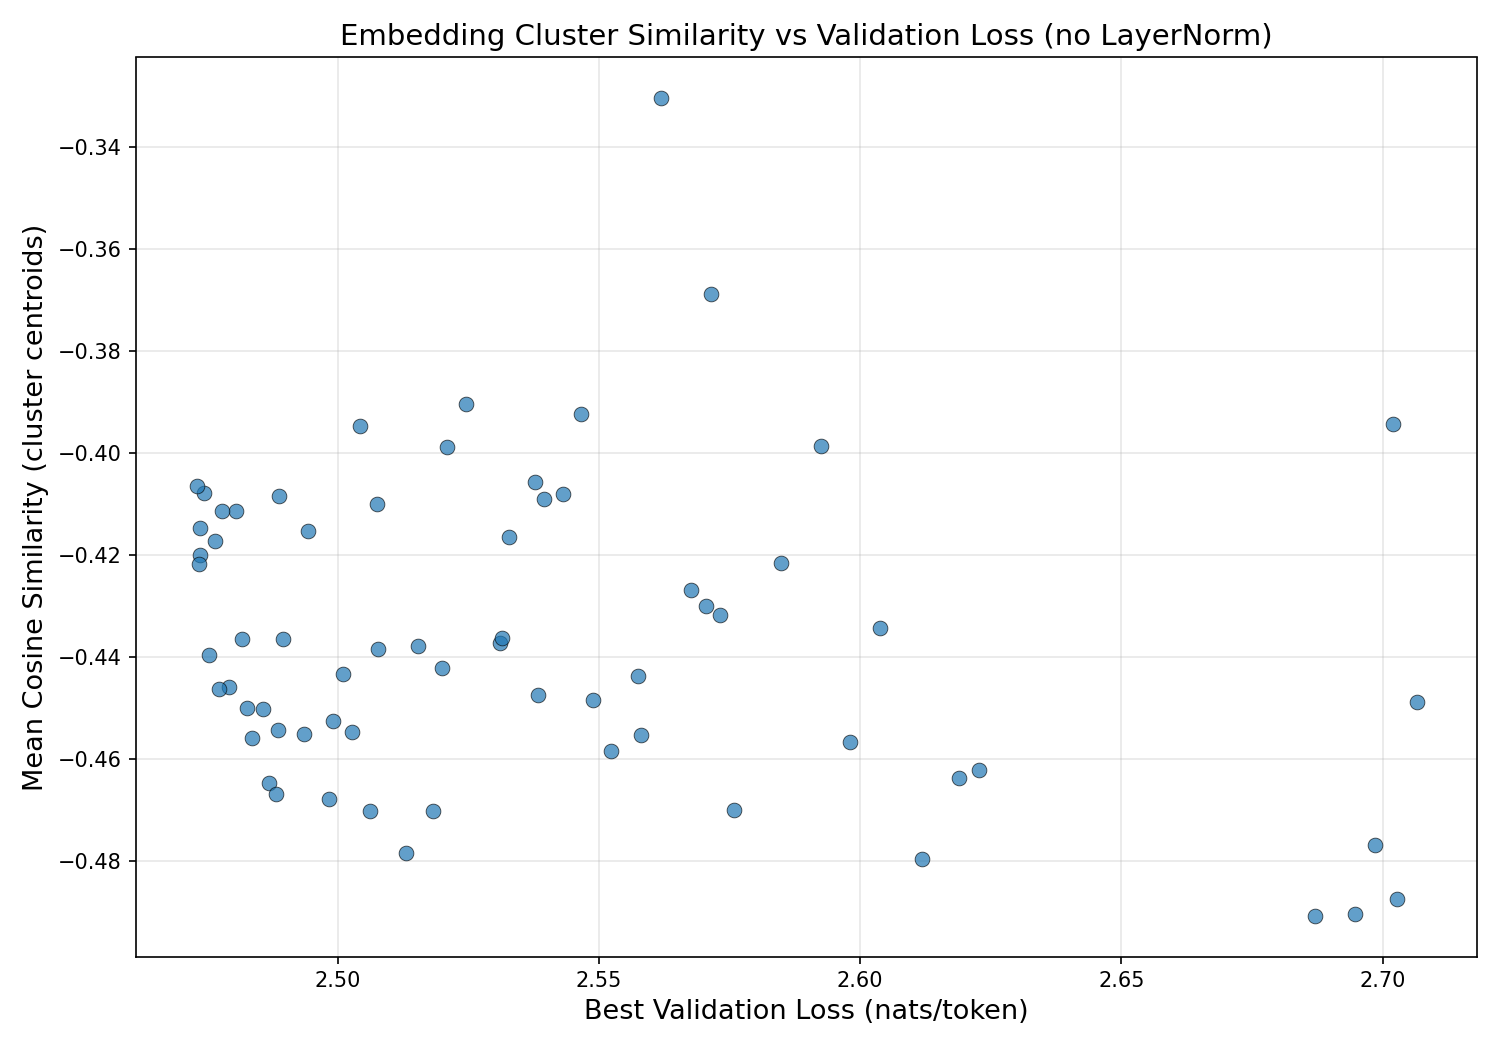
\includegraphics[width=\textwidth]{figures/embedding_cluster_similarity.png}
    \caption{Mean of the three pairwise similarities per model,
             restricted to architectures without LayerNorm (67~models).
             The trend is flat, with most models in $[-0.49, -0.35]$.}
    \label{fig:cluster-sim-mean}
  \end{subfigure}
  \caption{Cosine similarity between depth-cluster centroids of the
           embedding matrix versus best validation loss.
           (a)~Per-pair similarities for all models.
           (b)~Mean similarity for noLN models only.}
  \label{fig:cluster-sim}
\end{figure}

%----------------------------------------------------------------------
\section{Bayes-Optimal Loss at Finite Context}
%----------------------------------------------------------------------

The entropy rate $h$ is the minimum achievable loss for a predictor with
access to the infinite past.  A transformer with context window $T$,
however, can only condition on the most recent $T$ tokens.  To
disentangle the loss due to \emph{finite context} from the loss due to
\emph{limited model capacity}, we compute the Bayes-optimal next-token
loss at finite context: the best any predictor can do when restricted to
a window of length~$k$.

\paragraph{Setup.}
Let $\{X_t\}$ be the observed token process generated by the HMM with
hidden states $\{S_t\}$, transition--emission matrices
$E[v,s,s'] = P(X_t{=}v,\, S_t{=}s' \mid S_{t-1}{=}s)$, and stationary
distribution $\pi$.

Given a context window $(x_1,\dots,x_k)$, the Bayes-optimal prediction
for the next token is
\begin{equation}\label{eq:bayes-pred}
  P(X_{k+1}{=}v \mid x_1,\dots,x_k)
  \;=\; \sum_{s,s'} \alpha_k(s)\, E[v,s,s'],
\end{equation}
where $\alpha_k$ is the posterior (belief state) over hidden states after
processing the context.

\paragraph{Forward algorithm.}
The belief state is computed recursively via the forward algorithm.
Initialise from the stationary prior $\alpha_0(s) = \pi(s)$.  Upon
observing token $x_t$, update:
\begin{equation}\label{eq:forward}
  \tilde{\alpha}_t(s')
  \;=\; \sum_s \alpha_{t-1}(s)\, E[x_t, s, s'],
  \qquad
  \alpha_t(s') = \frac{\tilde{\alpha}_t(s')}
                      {\displaystyle\sum_{s''}\tilde{\alpha}_t(s'')}.
\end{equation}
The normalising constant $Z_t = \sum_{s'}\tilde{\alpha}_t(s')$ equals
the predictive probability $P(x_t \mid x_1,\dots,x_{t-1})$, so the
conditional log-likelihood of the context decomposes as
$\log P(x_1,\dots,x_k) = \sum_{t=1}^{k} \log Z_t$.

After $k$ update steps the belief $\alpha_k$ encodes all information
that the context provides about the current hidden state.  Plugging it
into Eq.~\eqref{eq:bayes-pred} yields the Bayes-optimal predictive
distribution and hence the minimum achievable loss at context length~$k$:
\begin{equation}\label{eq:Lstar}
  L^{*}(k)
  \;=\; \mathbb{E}\!\Bigl[
    -\log P\bigl(X_{k+1} \mid X_1,\dots,X_k\bigr)
  \Bigr],
\end{equation}
where the expectation is over sequences drawn from the HMM\@.

\paragraph{Fixed-context versus infinite-context.}
For a \emph{fixed} context window, each length-$k$ chunk is treated
independently: the belief is reset to $\pi$ at the start of every
window.  This is exactly the information available to a transformer with
context length~$k$.  For the \emph{infinite-context} baseline, the
forward algorithm runs over the entire sequence without resetting, so
the belief accumulates information from arbitrarily far in the past.
The difference
\begin{equation}
  \Delta(k) \;=\; L^{*}_{\text{fixed}}(k) - L^{*}_{\infty}
\end{equation}
isolates the cost of the finite context window.  As $k$ grows beyond the
mixing time of the chain, $\Delta(k) \to 0$.

\paragraph{Decomposing the transformer loss.}
The cross-entropy loss of a trained transformer $\hat{L}$ can now be
decomposed as
\begin{equation}
  \underbrace{\hat{L}}_{\text{transformer loss}}
  \;=\; \underbrace{h\vphantom{\hat{L}}}_{\text{entropy rate}}
  \;+\; \underbrace{\Delta(k)\vphantom{\hat{L}}}_{\text{finite-context cost}}
  \;+\; \underbrace{D_{\mathrm{KL}}\vphantom{\hat{L}}}_{\text{model capacity gap}},
\end{equation}
where $D_{\mathrm{KL}} = \hat{L} - L^{*}_{\text{fixed}}(k) \ge 0$
measures the sub-optimality of the transformer relative to the
Bayes-optimal predictor at the same context length.  Computing
$L^{*}_{\text{fixed}}(k{=}16)$ for the cylinder HMM will reveal how
much of the observed ${\sim}0.034$\,nat gap is attributable to finite
context versus limited model expressivity.

%----------------------------------------------------------------------
\section{Summary and Open Questions}
%----------------------------------------------------------------------

The cylinder graph HMM provides a controlled testbed for studying how
transformers learn to perform approximate Bayesian filtering over a
structured latent space.  Larger, deeper, full-architecture models
approach but do not reach the entropy rate, suggesting fundamental
limits tied to the autoregressive architecture and finite context.

Open directions include:
\begin{itemize}
  \item Characterising the belief-state geometry learned by the residual
        stream (cf.\ the fractal structure observed in the belief-state
        notebooks).
  \item Ablation studies on context length to quantify the loss
        attributable to finite $T$.
  \item Mechanistic interpretability of attention heads---do specific
        heads specialise in tracking depth transitions versus intra-layer
        dynamics?
\end{itemize}




\end{document}
